\documentclass[conference]{IEEEtran}
\usepackage{blindtext, graphicx}
\usepackage{listings}


\hyphenation{op-tical net-works semi-conduc-tor}

\title{Coflow Scheduling in data center networks}


\begin{document}

\author{ Stas Mushits, Amit Borase, Ruby Pai, Sreejith Unnikrishnan, Ritvik Jaiswal }

\maketitle


\begin{abstract}
%\boldmath
Current coflow schedulers require coflows to be explicitly identified by the programmer to the scheduler via an API. This is not ideal as it depends on the programmer manually identifying all coflows completely and accurately. This paper attempts to evaluate the performance of existing coflow schedulers in the case where coflows are incompletely identified.
\end{abstract}

\begin{IEEEkeywords}
Coflow scheduling, Data center networks
\end{IEEEkeywords}

\section{Introduction}

Data parallel cluster applications running on fast CPUs are limited by relatively slower network connections. Traditional network scheduling ignores application level requirements, focusing instead on metrics like flow completion time. The coflow abstraction for such applications was proposed in \cite{coflow}, which argued that identifying the parallel data flows associated with an application as a ``coflow'' and applying application-aware scheduling improves application performance.

Recently published coflow schedulers Varys \cite{varys} and Aalo \cite{aalo} focus on minimizing coflow completion time (CCT) as opposed to individual flow completion time. Varys and Aalo were shown to decrease average CCT by a factor of about 3 or 2 times, respectively. However, varys is clairvoyant in nature and requires the flows in a coflow to be identified to the scheduler via an API, whereas aalo is non-clairvoyant scheduler and doesn't need any coflow parameters to be declared to scheduler. Clairvoyant nature of varys puts additional burden on the programmer, and may not be realistic and possible in all cases: for example with legacy code, or there may be situations in which not all flows in a coflow are known to the programmer. However heuristic based aalo algorithm would be more pragmatic in real world networks. This project attempts to examine these schedulers as a function of knowledge of flows in a coflow.

\section{Related work}

The coflow abstraction represents a collection of related flows in a data network, and improving the coflow completion time is equivalent to improving the application performance. Minimizing coflow completion time (CCT) is a NP hard problem \cite{varys}, so schedulers like Varys \cite{varys} and Aalo \cite{aalo} use heuristics.

The Varys\cite{varys} scheduler uses a Smallest-Effective-Bottleneck-First (SEBF) heuristic, that schedules coflows based on its bottleneck flow`s completion time. Within each coflow, the Minimum-Allocation-for-Desired-Duration (MADD) algorithm is used to allocate rate for individual flows. MADD slows down all the flows in a coflow to match the completion time of the flow that will take the longest to finish. Combining SEBF and MADD effectively implements a heuristic that reduces average coflow completion time. In order to use SEBF and MADD, Varys must not only know the number of flows in a coflow, but their flow lengths in advance, making it clairvoyant scheduler.

However the authors proposed a new scheduling algorithm called Aalo\cite{aalo}, which is non clairvoyant, which in turn translates to a more pragmatic approach in coflow scheduling. Aalo uses multi-level queue structure. Observed coflow sizes are reported to the scheduler and used to determine when a coflow is demoted from one priority level queue to the next. The aalo scheduler uses a fixed coflow size threshold \(X\) for highest priority queue, and subsequent lower priority queues have thresholds multiplied by a factor of \(E^N\), where \(E\) is a constant and \(N\) is the priority level. All coflows enter the higher priority queue first. Within a queue, the scheduler follows a First In First Out (FIFO) principle. When the observed coflow size crosses the queue's threshold it gets de-prioritized into the next lower level queue. Weighted fair sharing across queues ensures that starvation of larger coflows does not occur.

\begin{figure}
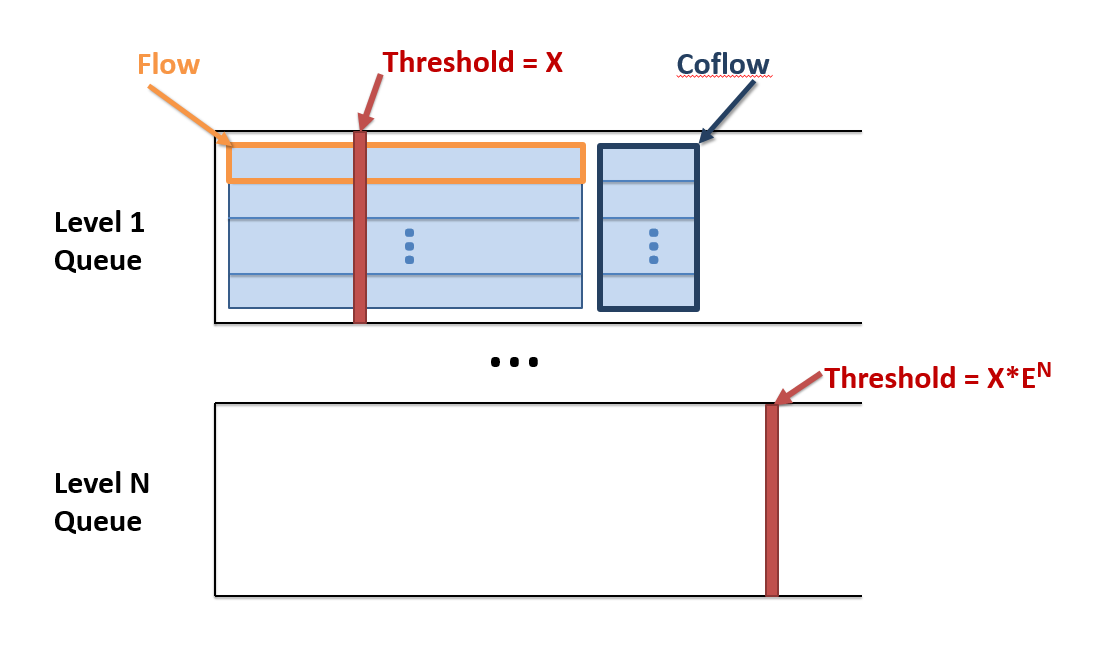
\includegraphics[width=0.5\textwidth]{queues.png}\caption{Scheduler Queues}
\end{figure}

%This ensures that shorter coflows will get effective bandwidth and is not greatly affected by larger flows. 
%Previous Orchestra, Baraat

\section{Design Decisions}

One of the preliminary task was to create a suitable environment to simulate and run the network. We did a survey of possible network simulators carefully looking for the features it provided and its suitability for our objective. For the baseline network simulation we decided to go for mininet\cite{Mininet}. There are other options like NS2 simulator etc. Support for python programming coupled with integration support with many VMs made our choice of picking up mininet easier. Moreover there is a huge community involvement and documentation for the tool.

The second decision was to decide on a network topology over which we should be running the simulation. Our aim was to ensure that rather than sticking to naive network topologies, we should rather read up on production quality network topologies, that is actually useful in real world scenario. Keeping that in mind and considering the pragmatic implications, we used fat-tree based network topology. Fat tree topology ensures that the end hosts receive full bisection bandwidth and there would be multiple path from a host to core server, ensuring higher bandwidth and reliability. Most of the fat tree implementation requires some method of hashing, usually ECMP to ensure that the multiple paths are effectively utilized. Our search for an SDN controller with ECMP support did not bear the fruit. The next best option was to find a controller that learns MAC addresses for efficient switching. Openflow Floodlight\cite{Floodlight} controller was selected for this purpose. Firstly floodlight supports learning based data forwarding and secondly provides Java based API. We were able to successfully create and deploy a fat tree topology with parameter K = 4, ensuring that we have 16 hosts connected to each other.

We ran the network in our allotted UCSD cluster machines. However we came across a problem when we tried to assign individual IP addresses to each mininet hosts. Mininet host will take IP`s based on the host name, which while running on a single VM is the same. To resolve this, we had to look for other means. After quite a bit of research, we decided to use Docker\cite{Docker} containers for deploying mininet hosts. Docker containers are essentially virtual machines without hypervisor. This essentially means that we were able to create Docker based software containers for individual mininet hosts and was deployed on our cluster virtual machines. Docket provide APIs that enables us to monitor, trigger and execute process in individual containers from the host machine. We used python based API for our interaction with docker containers.

Next step was to create software architecture that is efficient and flexible enough to create the simulation framework. Since the Varys and Aalo scheduler code runs on Scala, we decided to use Java as our main language. Given the legacy of socket programming and multi-threaded capability of Java, our choice proved effective in the long run. Our control traffic was handled in-band, with a master node. The system takes a hosts file that contains the list of hosts and their IP addresses as its input and a task file descibing the frame size, mapper reducer configuration etc. We also provide a simulation file in JSON format which the program uses to identify the Master URL, the URL where the Varys or Aalo scheduler listens to for scheduling the tasks. The Program then runs the simulation in accordance with the tasks file and produce relevant log files as the output. We created a small program in MATLAB, that would analyze the log files to generate graphs and results out of it.

\section{Design}

At the beginning of our research we decided to built a simulation system which would allow us to simulate data center traffic patterns on a small scale. As a network abstraction we chose Mininet. For host behaviour we tried decentralized and centralized system and chose centralized one because of it more predictable behaviour and easiness of deployment. Because of a dependency for a host name of a machine we chose Docker containers to run our hosts in.

\subsection{Simulating a network}
\subsubsection{Mininet}
Mininet is network emulation orchestration system, which creates a network of virtual hosts, switches, controllers, and links, that run on single Linux kernel underneath and share host file-system and other components. It uses lightweight virtualization to make a single system look like a complete network, running the same kernel, system, and user code. In short, mininet simulates all the hardware entities of network using software. Mininet exports powerful python API’s that could be used readily to design complex network topologies along with the required routing solution. We chose mininet to simulate network, mainly because of its fast deployability and customizability.

\subsubsection{Topology}
Fat-tree topologies are widely prevalent in today's data center network environments. Since the Coflow scheduling is largely effective in the isolated network environments such as data-centers, we decided to use fat-tree topology to simulate the data-center network. One of the many advantages posed by the fat-tree topology is the availability of multiple equal cost paths, but that meant we needed to write our own routing solution loosely based on the 2-level routing table solution\cite{fattree}. The strict time-constraint of the project meant we had to yield to a more ineffective routing solution such as ‘learning switch’, which does not take full advantage of all equal cost paths available and instead routes traffic through learnt paths only. 

Additionally, we tried to have an out-of-band and fast control network, but that meant we introduce loops in the topology and disturb the existing routing solution. Hence we decided to have an in-band control network by assigning the first host the sole role of scheduler and simulator controller. All our experiments were done on fat-tree topology with k-value of 4, that meant we had 16 hosts in the network.

\subsection{Simulation framework}
The next step was to create a program which could approximate the behaviour of a host in a datacenter. As we wanted to particularly inspect coflow behaviour our system, which should be very time sensitive, meaning that each flow should start in a specific point in time in order to give us ground for reasoning about its completion time and completion time of a coflow to which it belongs. We tried two approaches: decentralized and centralized system. For a network behaviour to simulate we chose MapReduce pattern since it is very common and very suitable for coflow usage.

\subsection{Decentralized system}
At first, we tried to build a decentralized system for simulation since it seemed more easy and faster to implement and should have been sufficient for our needs. It had one entity, we call it Actor since it plays a role assigned to it by simulation. Actors accepted configuration of simulation and tasks they need to accomplish and behaved based on that information. The task represented one flow and had starting time, sender, receiver and amount of data to transfer. Synchronization of timing among hosts wasn’t an issue because as programs deployed within mininet hosts they share kernel and use the same timer. 

Although this first system could behave using TCP sockets it we realized that it wasn’t very suitable for simulation of coflows since coflow should be registered by one host before other hosts can send traffic using this coflow. The situation was worsen by the need for generating of tasks for a simulation. As we wanted to simulate MapReduce we had to generate concrete tasks for each host so that part of the hosts in one specific moment would start behave as mappers and another part would start to behave as reducers. All of that required precise timing and generating task files for each host with this timing in mind which is as complex as a system itself.

\subsection{Centralized system}

\begin{figure}
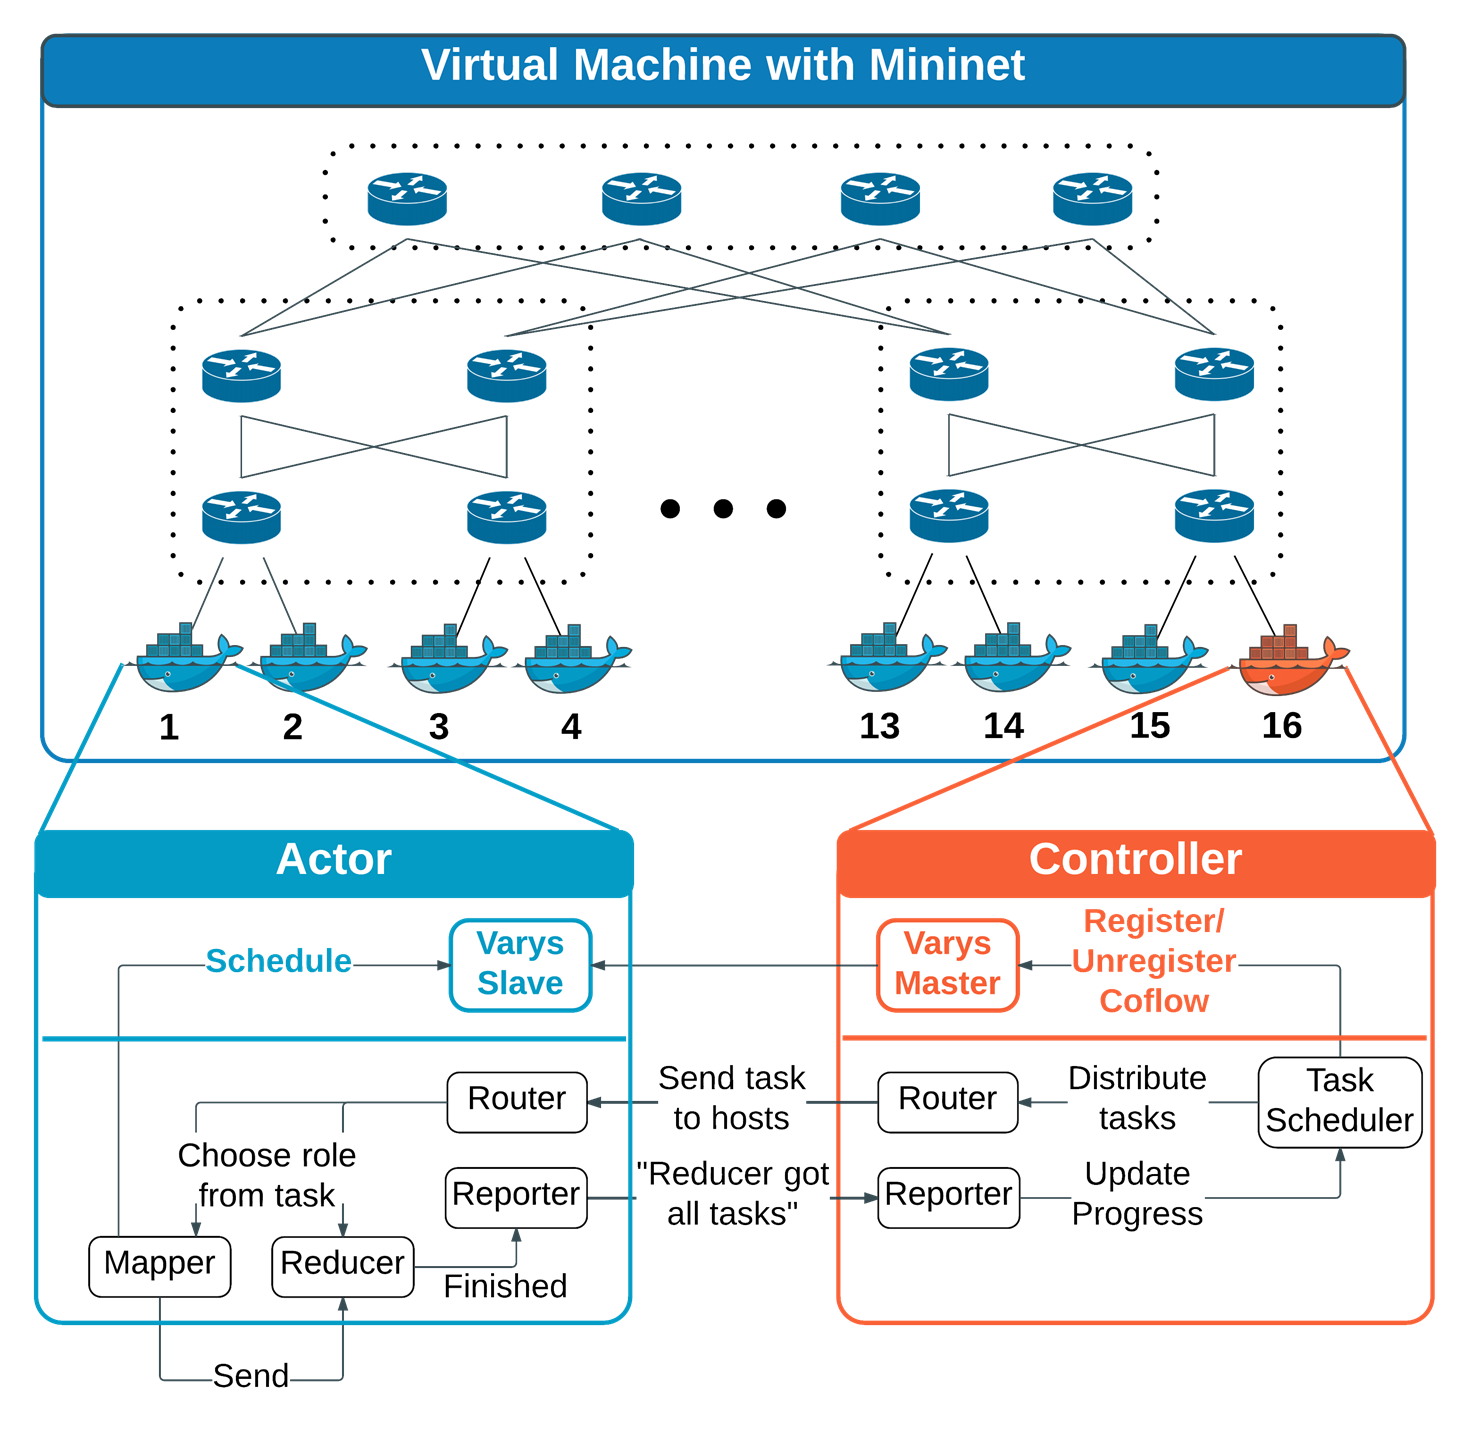
\includegraphics[width=0.5\textwidth]{setup.png}\caption{System Setup}
\end{figure}

Our second attempt was a centralized system with one Controller, which had all the tasks and knew about all other hosts in a network. It was deployed on a separate host in a network. With it we neglected the need to generate tasks for each host in the network separately, synchronize hosts by timing and could concentrate on the creating one task file which would allow us to easily coordinate behaviour of all Actors from the Controller.

The coordination and interaction between Controller and Actors as well as between Actors is the follows. On start of simulation Controller accept a task file which has the following format:

\begin{lstlisting}
Line 1: <Number of ports in the fabric> 
    <Number of coflows below (one per line)>
Line i: <Coflow ID> <Arrival time (ms)>
    <Number of mappers> <Location of map-m> 
    <Number of reducers> 
    <Location of reduce-r:Shuffle
    megabytes of reduce-r>
\end{lstlisting}

Task scheduler on the Controller then iterate through the tasks and send each task in appropriate time to all hosts which participate in execution of this task. Also, it register coflow for each task during the start of the task and unregister it when this task is finished.

Upon receiving the the task, Actor creates a mapper or reducer thread depending on a role given in a task. Using task mappers send specified amount of data to appropriate reducers using Aalo API which schedules sending using information on local Aalo slave and global Aalo master located on the Controller host. When reducer finishes receiving data from all mappers it report to Controller. When all reducers report to Controller about completion of the task Controller unregister coflow and measure its completion time.
Using this system we could vary the tasks, number of mappers and reducers, specify unlabeled flows in a coflow and orchestrate the whole system from one host. Also, the timing was simplified because only master knew when and which host should start sending or receiving and could activate all Actors in an appropriate order. 

\subsection{Docker containers as a mininet hosts}
During the initial phase of deployment with the coflow scheduler, we found out that the coflow scheduler heavily uses the hostname of the system to frame various control messages. Since the mininet hosts shared the file-system with the host, this posed a problem as the mininet hosts could not be configured to have a unique hostname across the virtual network, they merely had the same hostname as the underlying system. We tried to get-around this roadblock by designing a wrapper around the hostname API’s in java to return hostname that did not match with that of underlying host and were unique across mininet network. This approach did not prove to be fruitful as it required hard-coded hostname framing  at multiple places in both coflow scheduler code and the hosts system.  To get around this issue, we decide to have mininet hosts as docker containers.

Docker is an upcoming technology that allows packaging of an application with all of it’s dependencies into a single container, that works out-of-box and can be readily deployed on any docker environment regardless of the underlying hardware. Docker container thus built wrap up a piece of software along with a complete filesystem that contains everything it needs to run: code, runtime, system tools, system libraries. 

This meant that each docker container instance gets assigned a unique hostname, which ensured that we didn't needed to make any cosmetic changes to the coflow-scheduler code. Additionally  docker container allowed us to package both, coflow scheduler and simulator into a single image that could be readily uploaded and deployed on any machine as long as it ran Ubuntu system. This allowed us to carry out some of our experimentation on faster amazon EC2 instances without any additional setup requirements.

We used publicly available fork package of mininet \cite{dockernet} that replaces mininet hosts with docker containers.

\section{Experiment}

Our goal was to evaluate the impact of unlabeled flows within a coflow on the performance of state-of-the art coflow schedulers, in particular, on the metric of average coflow completion time (CCT). It is instructive to start with simple experiments whose results can be reasoned about, both to sanity check the correctness of the simulation setup and to gain insight, perhaps by uncovering unexpected behavior. 
To that end, we attempted to examine a scenario involving two coflows. We incrementally remove flow labels from one coflow and measure the impact of the second coflow as the percent increase in CCT compared to when the first coflow was properly labeled.

Our simple experiment involved one sender and ten receivers. We imagined a scenario in which two coflows, each with a corresponding width of ten flows, are being sent at the same time between the sender and the ten receivers, through the simulated fat tree topology. The nonclairvoyent Aalo scheduler uses observed coflow sizes in its scheduling decisions; in particular, when the observed coflow size crosses the threshold associated with a priority level, the coflow is demoted to the next lower priority level in its multilevel queue structure. Removing flow labels from a coflow effectively decreases the observed size of the coflow, allowing the incorrectly labeled coflow to retain a higher scheduling priority than intended for minimizing average CCT.

Within each queue, coflows are scheduled in FIFO order. In order to see the impact of incorrectly labeling one coflow on a second coflow, the incorrectly labeled coflow arrives at the scheduler before the coflow being impacted, and also has a total size much larger than the threshold of the highest priority level queue. For simplicity, the second coflow has a total size that allows it to retain the highest level priority.

We collected CCT data for simulations of this scenario, as well as two additional simple scenarios involving smaller coflows being blocked by the incorrectly labeled larger coflow which was allocated an incorrect share of network time. The other scenarios involved increasing the number of smaller coflows and also smaller coflows of different sizes.

We scaled the first level queue coflow size threshold and multiplier on thresholds of lower level queues to match the data sizes that we were able to accommodate comfortably with our simulation code (from a first level queue threshold of 10 MB to 1MB, and a multiplier $E=10$ to $E=2$). We discovered after our data collection, however, that the a parameter in the Aalo scheduler software should have been adjusted correspondingly for small size flows to be registered with the scheduler at all. The net effect was that the smaller coflow was not being managed by the scheduler and our experiment did not occur as intended. Time constraints, coupled with the large amount of time required to collect one single run of each experiment with our setup, meant we did not have time to collect the intended data.

The results of our data collection for the simple two coflow scenario are shown below. Because of the error in our experimental setup, these graphs mainly show how we intended to visualize the results. 

\begin{figure}
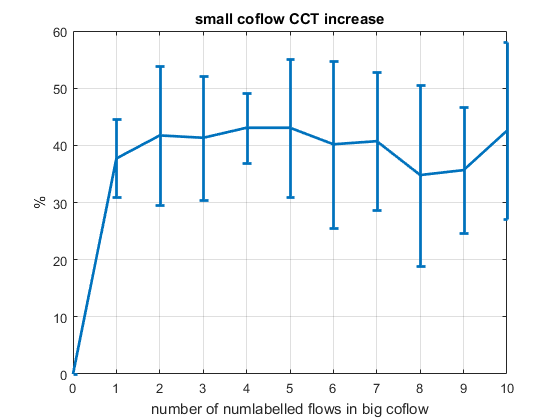
\includegraphics[width=0.5\textwidth]{smallcoflow.png}
\label{figure:smallcoflow}
\end{figure}

\begin{figure}
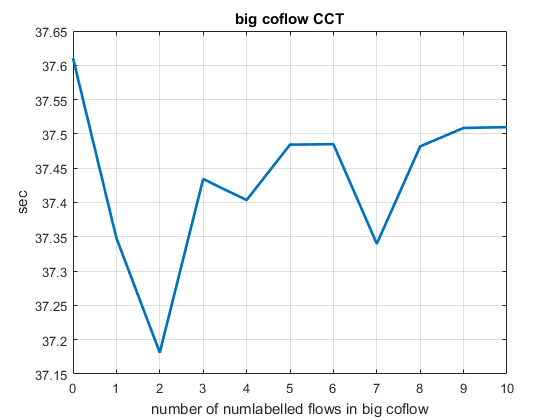
\includegraphics[width=0.5\textwidth]{bigcoflow.png}
\label{figure:largecoflow}
\end{figure}

Analytically, if $m$ is the number of flow labels removed from a total of $M$ flows in the large coflow, its observed size would be $\frac{M-m}{M}$ of its actual size, so it would stay at a priority level $\frac{M}{M-m}$ longer than it should. We would expect the small coflow's CCT to increase correspondingly with increasing $m$.

\begin{figure}
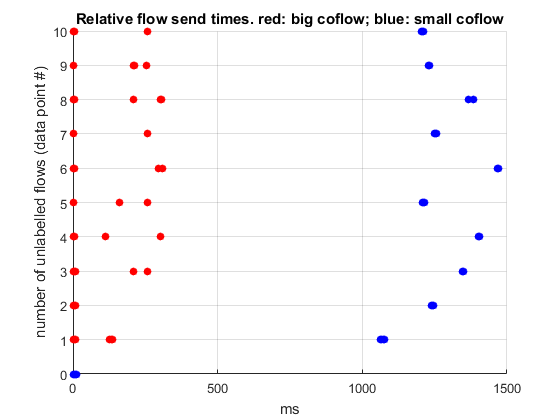
\includegraphics[width=0.5\textwidth]{sendtimes.png}
\end{figure}

In addition, we examined the send times for the individual flows in our experiment, one example of which is pictured below. This was a useful tool for debugging earlier iterations of the simulation software. For any given experiment (vertical axis), the flows in the large coflow should have been sent at approximately the same time, but we observe variation of up to hundreds of milliseconds, which is on the order of the variation in CCT observed for the large coflow.

Given these observations, a next step would have been to quantify the and perhaps attempt to remove some of the timing inaccuracy of our control over and measurements of timing, which would be essential to gathering good results.

The simple experiments just described would have given us insights to design workloads appropriate to our simulation setup to evaluate impact of incompletely identified coflows on average CCT over a large number of coflows competing for cluster bandwidth.

\section{Conclusion}

A mininet simulation environment and control software were created to study the performance of coflow scheduling with incompletely identified coflows. This involved extensive study of parts of the Varys and Aalo scheduler code bases as well as solutions to mininet limitations. The simulation software involved hundreds of man-hours of development. One takeaway is that software to support research goals should, besides following a spiral development process, support only the functionality needed for the experiment at hand, rather than attempting to anticipate and support future complex scenarios.

In addition, another approach to the goal of studying coflow scheduling with incomplete coflow identification might have been to understand analytically how removing flow labels impact coflow completion times under existing coflow scheduling algorithms, both of correctly labeled coflows in small examples and for the average CCT of a workload. Insights could then be applied to attempting to modify the scheduler algorithm or parameters to accommodate incompletely identified coflows.

\section*{Acknowledgment}
We would like to thank our instructor Prof. George Porter for his support through out the project and his valuable insights over time. We also would like to thank our TA Yashar for helping us many a times. 

\begin{thebibliography}{99}

\bibitem{aalo}
Efficient Coflow Scheduling Without Prior Knowledge, 
\textit{Mosharaf Chowdhury and Ion Stoica, SIGCOMM, 2015.}

\bibitem{varys}
Efficient Coflow Scheduling with Varys, 
\textit{Mosharaf Chowdhury, Yuan Zhong and Ion Stoica, ACM SIGCOMM, 2014.}

\bibitem{coflow}
Coflow: A Networking Abstraction for Cluster Applications, 
\textit{Mosharaf Chowdhury and Ion Stoica, ACM Hotnets, 2012.}

\bibitem{Mininet}
Mininet - rapid prototyping for SDN
\textit{https://github.com/mininet/mininet}

\bibitem{Floodlight}
Flood light SDN controller
\textit{https://github.com/floodlight/floodlight}

\bibitem{Docker}
Docker
\textit{https://www.docker.com/}

\bibitem{dockernet}
Dockernet
\textit{https://github.com/mpeuster/dockernet}

\bibitem{fattree}
A scalable, commodity data center network architecture, 
\textit{Mohammad Al-Fares, Alexander Loukissas and Amin Vahdat, SIGCOMM, 2008.}

\end{thebibliography}


\begin{IEEEbiography}[{\includegraphics[width=1in,height=1.25in,clip,keepaspectratio]{picture}}]{John Doe}
\blindtext
\end{IEEEbiography}

\end{document}


